\chapter{Experimentos}
Debido a que el trabajo tiene dos partes principales, claramente diferenciadas, se han diseñado distintos tipos de experimentos para la evaluación de cada parte: un conjunto de experimentos en simulación para probar el rendimiento de los algoritmos de aprendizaje por refuerzo y un conjunto experimentos en real para probar la plataforma hardware y el diseño del autopiloto.
\section{Experimentos en simulación}
Con el ánimo de probar los distintos algoritmos de control basados en aprendizaje por refuerzo, se han diseñado diversos experimentos para comparar el rendimiento de estos algoritmos con el de un PID clásico. 
\subsubsection{Control en 1 GdL (\textit{Roll})}

En este experimento se comparan en rendimiento de los algoritmos PPO, DDPG , TRPO y PID para estabilizar la aeronave en \textit{roll}, restringiendo el movimiento de los otros ejes. 

\begin{figure}[htb!]
	\centering
	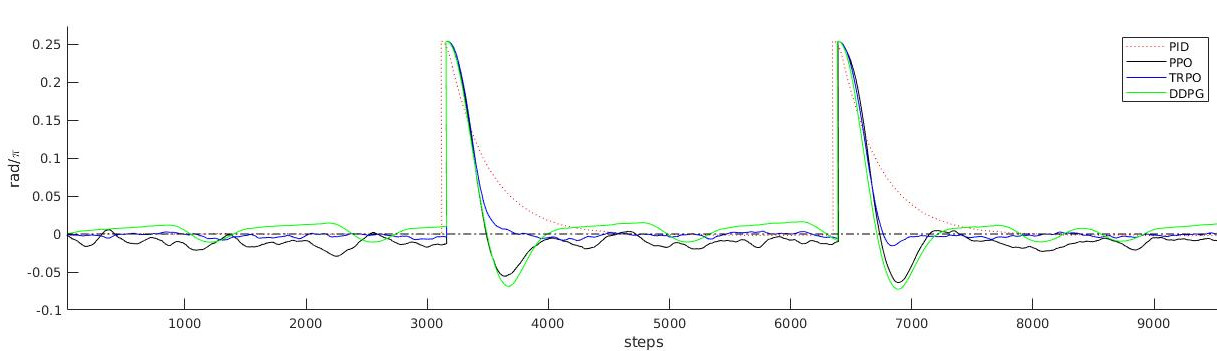
\includegraphics[width=\textwidth]{experimentos/sim_onlyroll}
	\caption{Estabilización en \textit{roll} en un entorno simulado.}
	\label{mat_lab_graph}	
\end{figure}

En este experimento, se observa como el TRPO consigue una mejor respuesta que el resto de los algoritmos. El PPO y el DDPG generan comportamientos similares.
\newpage 
\subsubsection{Control en 1 GdL (\textit{Pitch})}

En este experimento se comparan en rendimiento de los algoritmos PPO, DDPG , TRPO y PID para estabilizar la aeronave en \textit{pitch}, restringiendo el movimiento de los otros ejes. 

\begin{figure}[htb!]
	\centering
	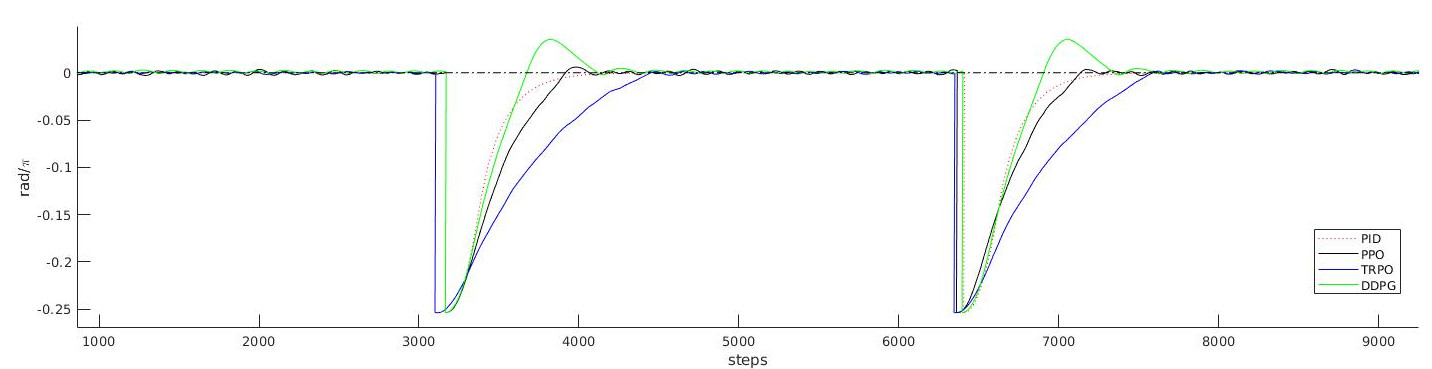
\includegraphics[width=\textwidth]{experimentos/sim_onlypitch}
	\caption{Estabilización en \textit{pitch} en un entorno simulado.}
	\label{mat_lab_graph}	
\end{figure}

En este experimento, se observa como el PPO consigue una mejor respuesta que el resto de los algoritmos. En este entrenamiento el TRPO consigue un peor rendimiento frente a los demás.


\subsubsection{Control en los 3 GdL}

En este experimento se comparan en rendimiento de los algoritmos PPO, DDPG , TRPO y PID para controlar la estabilización completa en los 3 ejes. 

\begin{figure}[htb!]
	\centering
	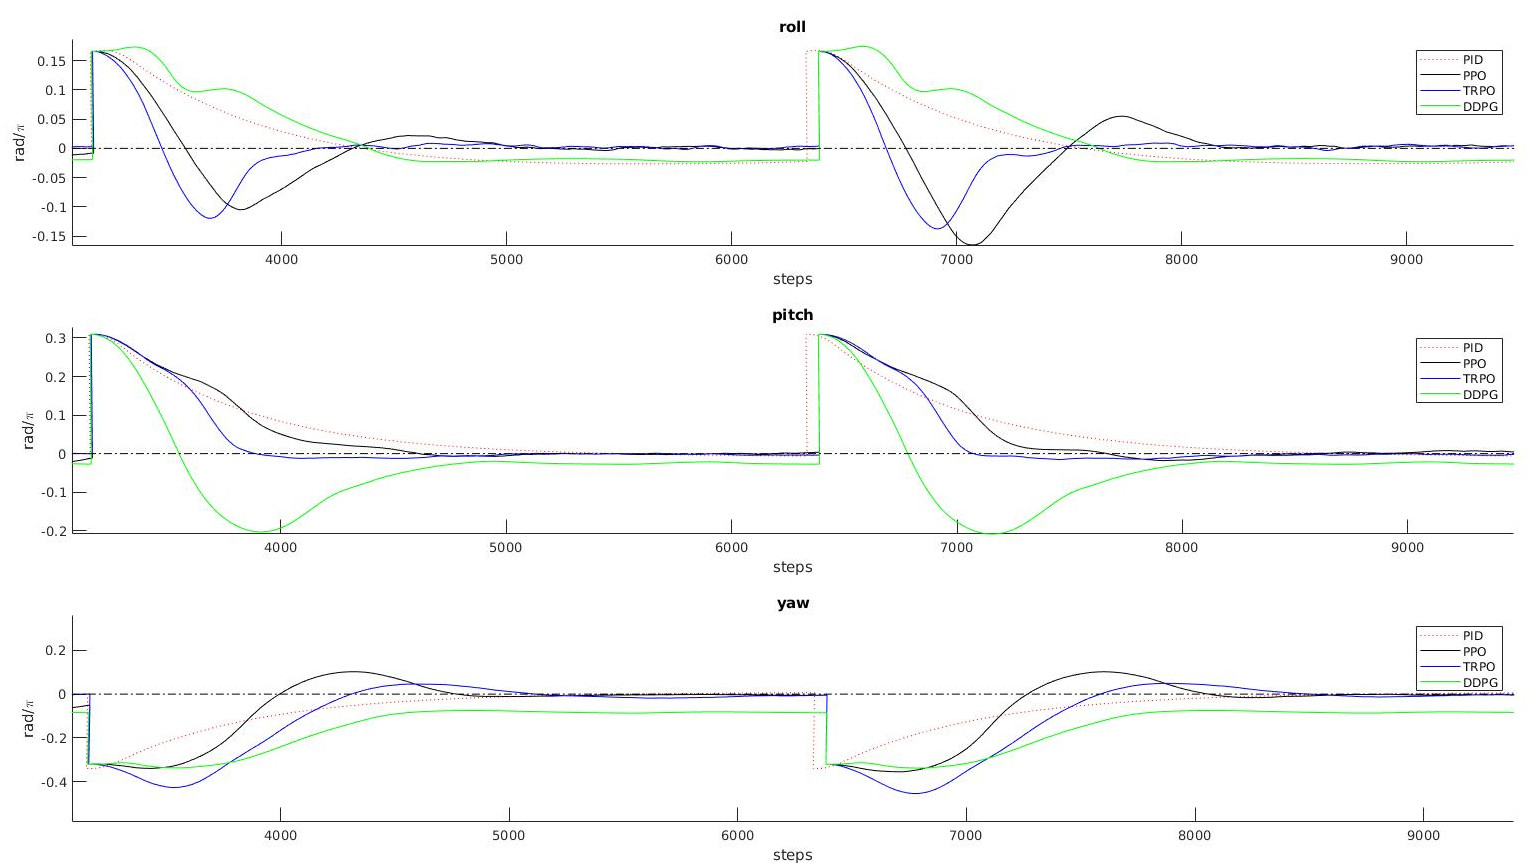
\includegraphics[width=0.9\textheight,angle=90]{experimentos/3_angles_real}
	\vspace{0.5cm}
	\caption{Estabilización en \textit{roll}, \textit{pitch y \textit{yaw}} simultáneamente}
	\label{Fig.7.2}	
\end{figure}

En este experimento, se observa como el TRPO consigue una mejor respuesta que el resto de los algoritmos, mostrando una salida mucho más rápida . El PPO sobreoscila demasiado en \textit{roll} y presenta un error de posición, véase en la \Cref{Fig.7.2}

\section{Experimentos en real}
Para la evaluación de la plataforma de vuelo , el diseño del cuadricóptero y del autopiloto, se han realizado distintos experimentos para intentar controlar la aeronave con algoritmos PID en cascada a una frecuencia de 70Hz.
\subsubsection{Control en 1 GdL (\textit{Pitch})}

En este experimento (\Cref{mat_lab_}) se ha empleado la rótula de 1 GdL que únicamente permite el movimiento en \textit{pitch}.

\begin{figure}[htb!]
	\centering
	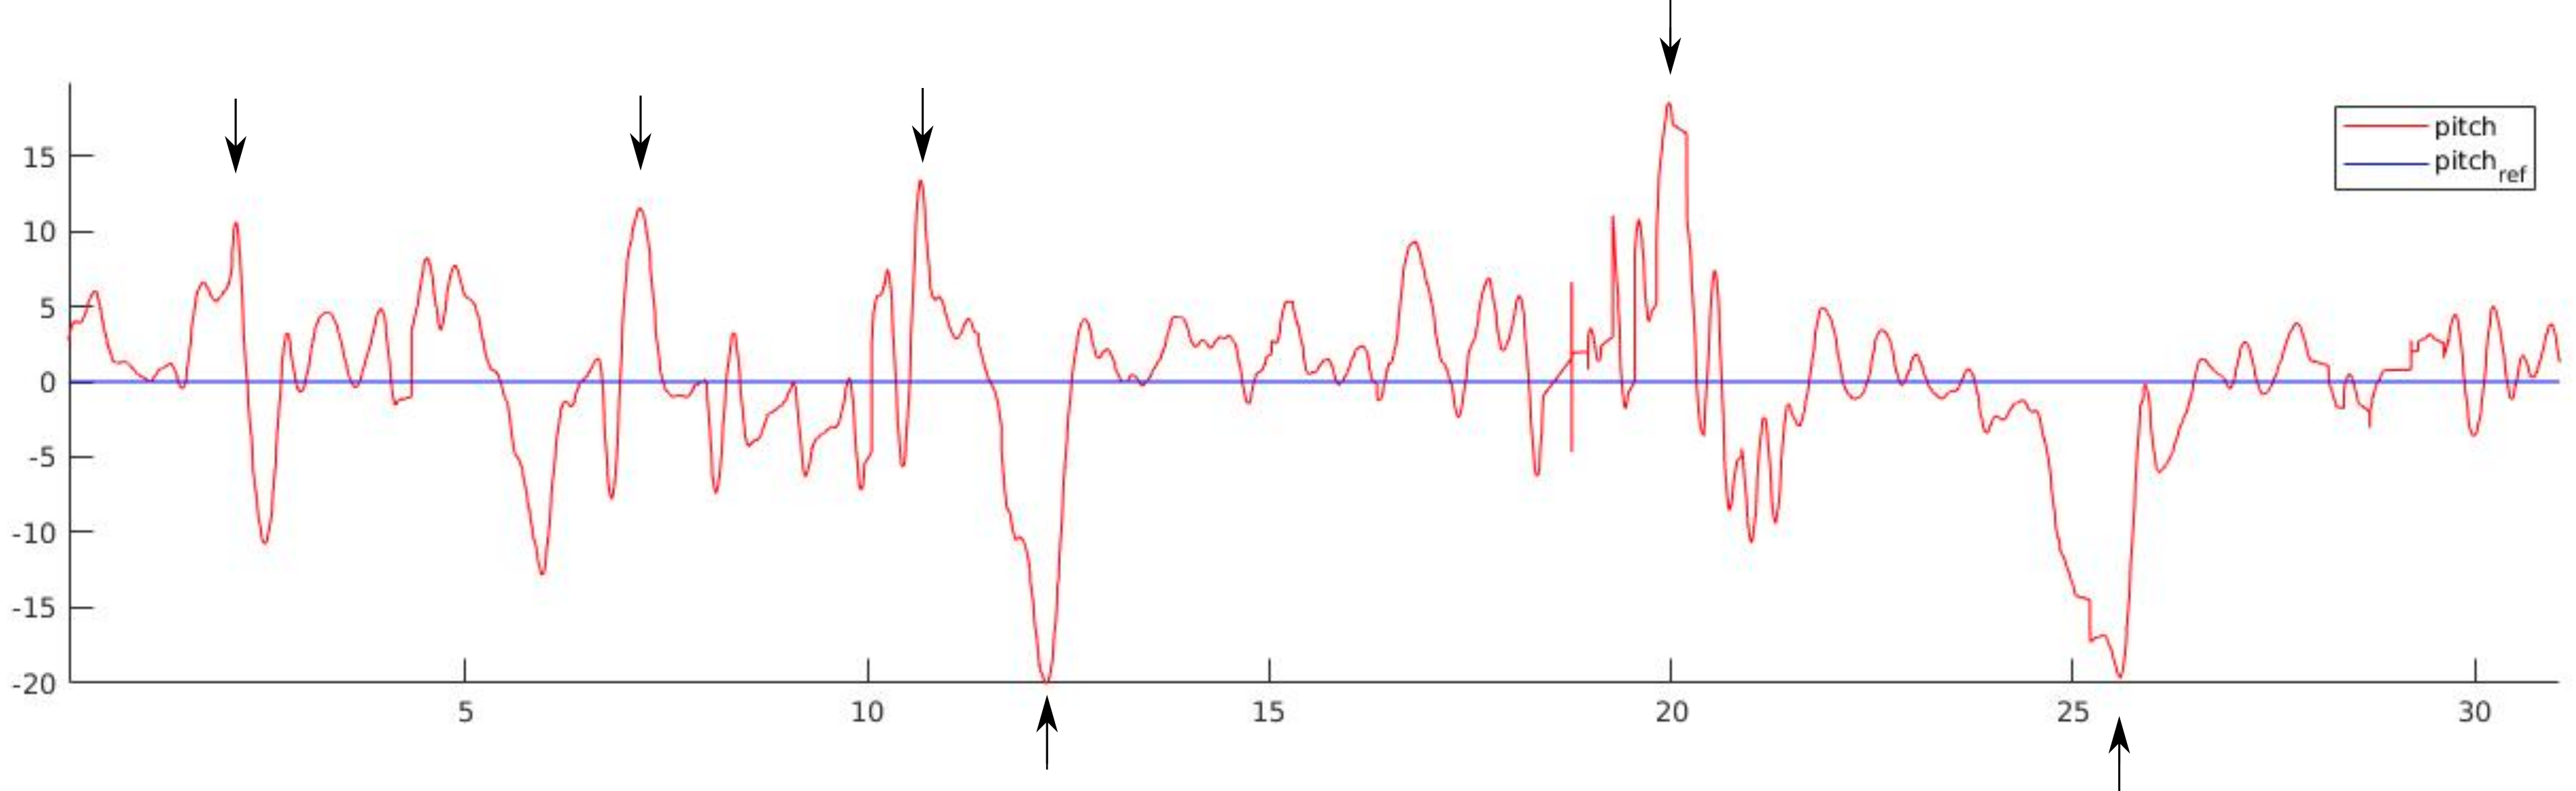
\includegraphics[width=\textwidth]{experimentos/real_only_pitch}
	\caption{Estabilización en \textit{pitch}. Las flechas marcan los tiempos en los que se perturbó al sistema.}
	\label{mat_lab_}	
\end{figure}

Se observa que el sistema es capaz de estabilizarse y que reacciona ante las perturbaciones externas de forma ágil. Por otro lado, también podemos observar ruido en la zona estable, además de poseer un pequeño error de posición de unos 2\grad.

\begin{figure}[htb!]
	\centering
	\includegraphics[width=\textwidth]{experimentos/time_lapse_pitch_real}
	\caption{Estabilización en \textit{pitch}}
	\label{tl_pr}	
\end{figure}


\subsubsection{Control en 1 Gdl (\textit{Roll})}
En este experimento (\Cref{mat_lab_gra})se ha empleado la rótula de 1 GdL que únicamente permite el movimiento en \textit{roll}.

\begin{figure}[htb!]
	\centering
	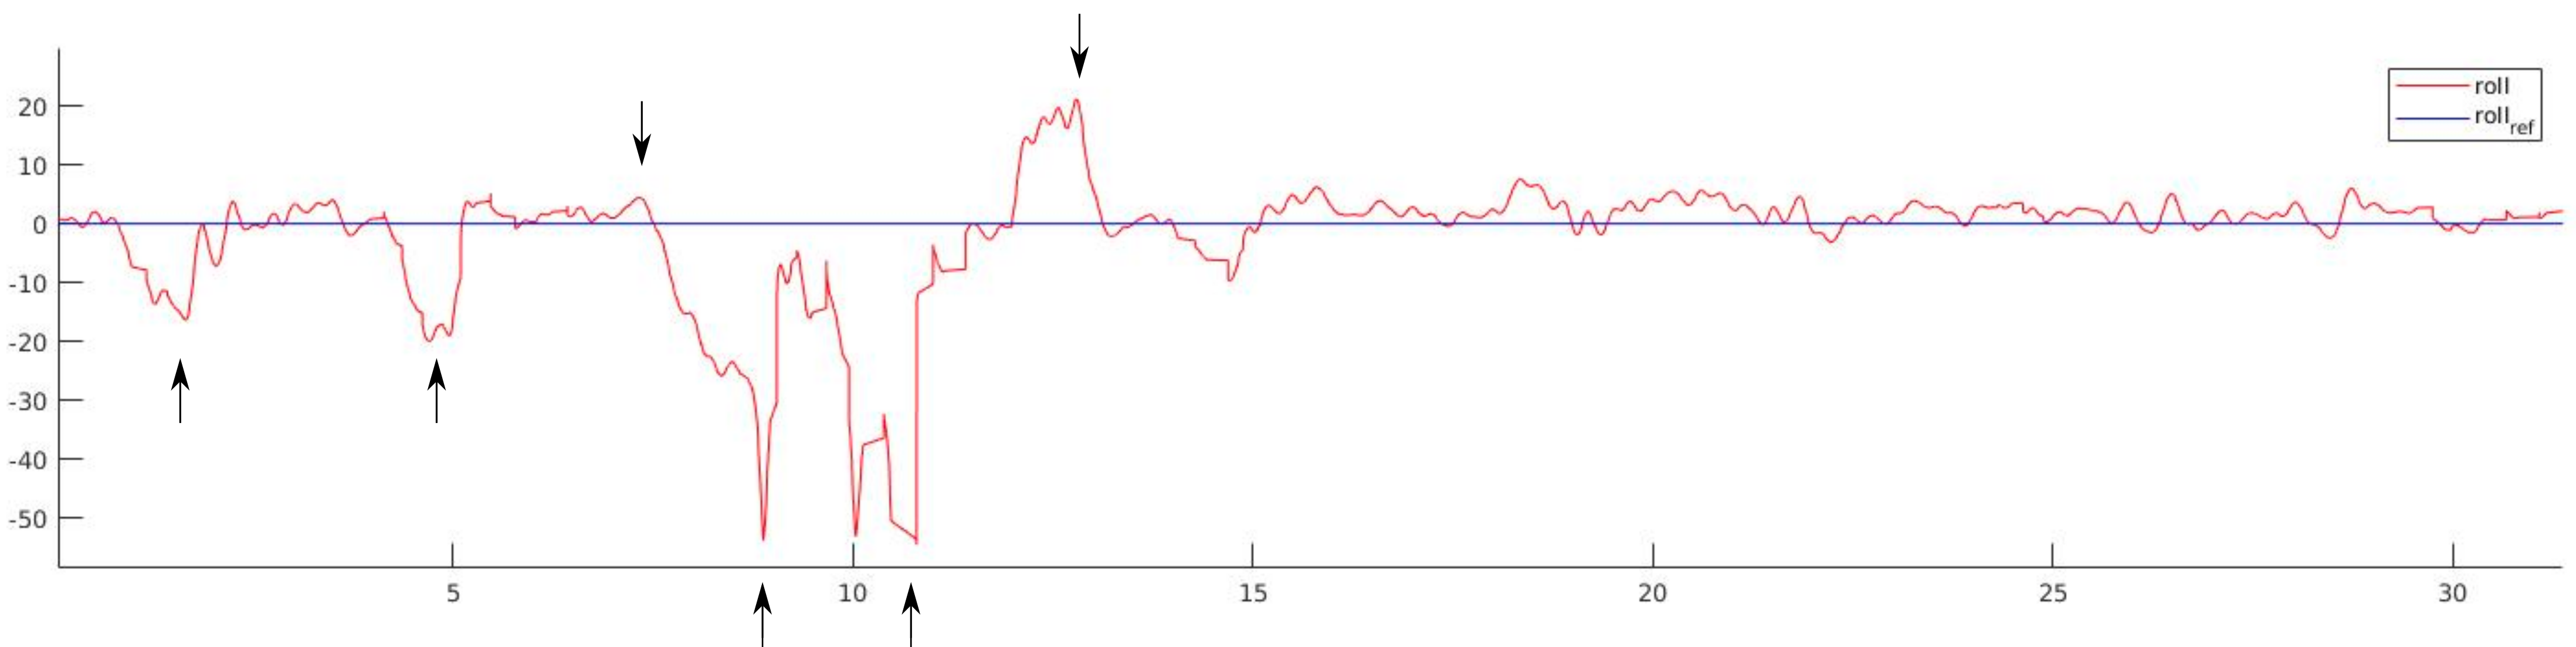
\includegraphics[height=0.18\textheight,width=\textwidth]{experimentos/real_only_roll}
	\caption{Estabilización en \textit{roll}. Las flechas marcan los tiempos en los que se perturbó al sistema.}
	\label{mat_lab_gra}	
\end{figure}

\begin{figure}[htb!]
	\centering
	\includegraphics[width=\textwidth]{experimentos/timelapse_roll}
	\caption{Estabilización en \textit{roll}}
	\label{tl_pr}	
\end{figure}

El comportamiento observado es similar al del experimento anterior: el sistema se estabiliza y consigue llegar a la referencia después de perturbarlo de una forma ágil, pero también se observa ruido y un pequeño error de posición en el régimen permanente.

\subsubsection{Control en los 3 Gdl}

En este experimento se ha empleado la rótula de 1 GdL que permite el movimiento en \textit{roll}, \textit{pitch} y \textit{yaw} .
\\

En este experimento (\Cref{tl_p1r}) observamos que aumenta el ruido que encontramos en el régimen permanente en \textit{pitch} y en \textit{roll}, aunque se disminuye el error de posición que veíamos en los experimentos anteriores. Por otro lado el controlador de \textit{yaw} es el menos ruidoso, pero también el más lento.

\begin{figure}[htb!]
	\centering
	\includegraphics[width=\textwidth]{experimentos/timelapse_yaw}
	\caption{Estabilización en los 3 ejes}
	\label{tl_pr}	
\end{figure}


\begin{figure}[htb!]
	\centering
	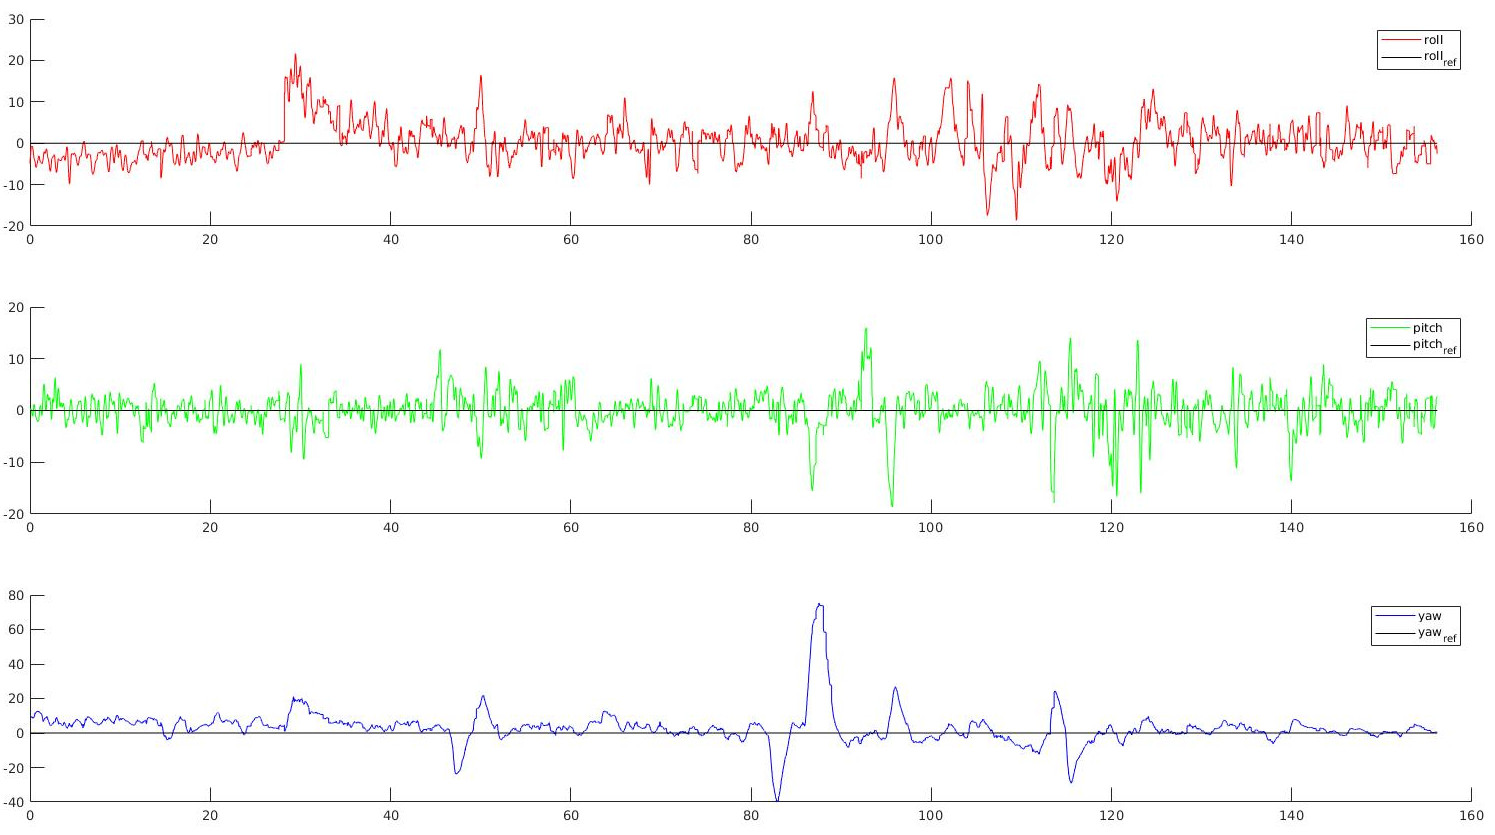
\includegraphics[width=0.9\textheight,angle=90]{experimentos/3_in_one_matlab}
	\vspace{0.5cm}
	\caption{Estabilización en \textit{roll}, \textit{pitch y \textit{yaw}} simultáneamente}
	\label{tl_p1r}	
\end{figure} 
%\begin{figure}[htb!]
%	\centering
%	\begin{tabular}{|c|c|c|c|}
%	\hline
%	&$K_p$&$K_i$&$K_d$\\
%	\hline	
%	$PID_{\dot\varphi}$ &0.003 & 0.0002  & 0.004\\
%	\hline
%	$ PID_{\dot \theta}$ &0.003 & 0.0002  & 0.004\\
%	\hline
%	$ PID_{\dot \psi}$ &0.003 & 0.0002  & 0.004\\
%	\hline
%	\end{tabular}\\
%
%\end{figure}